% !Mode:: "TeX:UTF-8"
\chapter{SNO+实验的位置重建以及UQ}

探测器中收集到的原始数据无法直接拿来做物理分析,这些数据需要经过
一系列的计算,才能拿到后续所需要的物理量。例如经过计算拿到了衰变顶点
的位置,方向,能量,粒子类型等,并进行分析。这一计算过程我们称之为重建。

这一章首先\ref{sec:classical_reconstruction}节介绍SNO+探测器中传统的重建方法,即最大似然法。
接着在\ref{sec:dl_reconstruction}节介绍深度学习在SNO+探测器中的重建方法,并给出两者结果的比较。

同时也会给出两者重建结果不确定性的估计。

\section{SNO+探测器中传统的位置重建方法}\label{sec:classical_reconstruction}

在SNO+探测器中,传统的重建方法主要是基于MLE (Maximum likelihood estimation,
最大似然估计)的。一般我们通过PMT的时间和位置信息来进行重建。可能后期还会
加入其他的信息,例如PMT的积分电荷等。SNO+实验中应用的MLE方法是基于一个假设,
即PMT接收到了一个内部电子的光子信号。\cite{anderson2024}虽然这个假设可能不是
一直成立,不过我们还会用其他的方法来分辨粒子类型。

更严谨地说,如果我们想确定一个事件的位置,我们会把一个基于时间残差的似然
函数在每个PMT上最大化。时间残差$T_{res,i}$的定义为:
\begin{equation}
T_{res,i} = T_{PMT,i}-T_{fit}-T_{transit}(\vec{x}_{PMT,i},\vec{x}_{fit})
\label{eq:residual}
\end{equation}
其中$T_{PMT,i}$为PMT被击中的时间,$T_{fit}$为事件的拟合时间,$T_{transit}$为光子在PMT和事件之间传播的时间。
一般我们认为光子沿直线传播,所以$T_{transit}$可以表示为:
\begin{equation}
T_{transit}(\vec{x}_{PMT,i},\vec{x}_{fit}) = \frac{||\vec{x}_{PMT,i}-\vec{x}_{fit}||}{c_{avg}}
\end{equation}
其中$c_{avg}$为光子在液体闪烁体中的平均速度。
不过在SNO+中,光子需要穿过液体闪烁体,AV,UPW和PMT的玻璃等介质,才能到达
PMT的收集装置。

$T_{res,i}$的分布一般服从正态分布,其均值为0,方差为$\sigma_{i}^2$。所以似然函数可以表示为:

完整的PDF (Probability density function,概率密度函数) 由于考虑了
反射,PMT本身的噪声以及各种其他的效应,更加的复杂。结果为一个具有长尾巴
并且有多个峰的分布。这个结果是从模拟和刻度中得到的。\cite{anderson2024}

$T_{fit}$ 和 $x_{fit}$是我们需要拟合的参数。我们可以通过最大化似然函数来得到它们的值。
\begin{equation}
\mathcal{L}_{vertex} = \prod_{i=1}^{Nhits} P(T_{res,i})
\end{equation}

其中Nhits是PMT被击中的数目。不过一般来说,我们不会直接最大化似然函数,而是最小化负对数似然函数:

\begin{equation}
-log(\mathcal{L}_{vertex}) = -\sum_{i=1}^{Nhits} \log P(T_{res,i})
\label{MLE}
\end{equation}

更具体一点,SNO+使用的是Powell算法\cite{powell1964efficient}来最小化负对数似然函数。
Powell算法是一种无导数的优化算法,它通过迭代地调整参数来找到函数的最小值。该算法使用了一个线性组合的搜索方向,
并在每次迭代中更新参数。Powell算法的优点是它不需要计算梯度,因此适用于那些难以计算导数的函数。
例如SNO+目前重建所用的PDF。当然,不止传统算法,
神经网络在训练时的梯度下降算法的思想与Powell算法比较相似。

目前SNO+实验所使用的重建方法涉及各种算法的先后结合。主要算法如\ref{MLE}
一样最小化负对数似然函数来确定事件位置。然而,尽管最大化似然函数是该过程中的第一步,
由于需要拟合的参数必须初始化为某个值,有几个算法是事先运行的。
这个被初始化的值通常称为种子。与神经网络反向传播的情况一样,初始值对是否能准确重建有很大的影响。

我们使用的初始化算法基于只需要4个PMT击中就可以解析地计算事件的位置和时间的原理。
根据\ref{eq:residual},$T_{res,i}$设置为零时有四个参数需要拟合,所以只需要四次命中PMT的信息。
当然,在实际应用中,计算位置和时间的准确性取决于选择哪四个PMT,光子从事件到击中PMT的路径,
以及与击中时间相关的噪声。

\section{深度学习在SNO+探测器中的位置重建方法}\label{sec:dl_reconstruction}

上面我们简要介绍了传统的位置重建方法,我们可以看到,传统的方法需要对PMT的响应进行建模,
并且对噪声和背景有较强的依赖性。而深度学习方法则是基于数据驱动的方法,
通过对大量实验数据的学习,可以捕捉到一些传统方法捕捉不到的信息并进行事件重建,
具有更好的适应性和鲁棒性。

接下来我们介绍深度学习在SNO+探测器中的位置重建方法。前面\ref{intro-NN}节中介绍了神经网络的基础架构,
以及CNN和RNN,这两种神经网络在粒子物理实验的重建工作中都有使用。
我们使用的是在\ref{transformer}节中介绍的\textbf{Transformer}模型。
得益于Transformer模型的自注意力机制,
我们可以在输入数据中捕捉到长距离的依赖关系,从而更好地建模复杂的事件特征。

\section{数据集}\label{dataset}

我们在\ref{summary}节中提到,我们使用了SNO+实验的模拟数据集来训练和测试模型。
主要为了保证模型的泛化能力,我们使用了不同的能量范围和位置的数据集。
主要使用了${}^{8}B$衰变道的太阳中微子数据。
这里与之前SNO+组内使用的模拟数据不同的是,我们额外使用了不同探测器状态的模拟,
以此来保证模型的泛化能力。\footnote{在SNO+实验中,探测器在不同的时间有不同的状态,例如在
某些时候,探测器的某些PMT会关闭,或者会进行维护,这些状态会影响PMT的响应。}
而SNO+合作组使用的RAT (Reactor analysis tool,反应堆分析工具)
软件提供的MC框架中提供了完整的run-by-run的模拟数据设置。也就是说,
模拟可以完整包含对应run number的所有的PMT状态信息。这大大提升了训练出来的模型的鲁棒性,
使得我们在预测时,即使在不同的探测器状态下也能有较好的效果。

我们的模拟使用的是SNO+中液体闪烁体阶段的探测器。其液体闪烁体配方为LAB+PPO+bis-MSB。
在模拟完成后,我们提取对于位置重建有用的信息,如PMT的时间和位置,
以及真实的事件位置,能量等。我们使用了大约$10^6$个事件来训练模型,分为训练集和测试集。
训练集和测试集的比例为70\%和20\%。

\section{位置重建模型架构}\label{model_architecture}

我们采用基于Transformer的模型进行位置重建。该模型主要包括特征嵌入、Transformer编码器和输出层。

\subsection{输入与嵌入}
模型的输入是每次事件中被触发的光电倍增管 (PMT) 的命中序列。每个命中包含时间、PMT ID及其三维坐标 (x, y, z) 。这些原始特征首先被转换 (嵌入) 为固定维度的向量。连续特征 (时间、坐标) 通过线性层处理,分类特征 (PMT ID) 通过查找表转换。所有特征的嵌入向量被拼接起来,形成每个命中的初始表示。

\subsection{Transformer编码器}
嵌入后的命中序列被送入Transformer编码器。在进入编码器之前,会添加位置编码以保留命中顺序信息。编码器由多个堆叠的注意力模块 (Attention Block) 组成。每个模块包含:
\begin{itemize}
    \item \textbf{多头自注意力 (Multi-Head Self-Attention) }: 捕捉序列中不同PMT命中之间的复杂关联。
    \item \textbf{前馈神经网络 (Feed-Forward Network) }: 对注意力层的输出进行进一步处理。
\end{itemize}
每个模块都使用了层归一化 (Layer Normalization) 和残差连接 (Residual Connection) 来稳定训练和提升性能。

\subsection{输出层与损失函数}
编码器处理完整个序列后,输出每个命中位置的上下文感知表示。为了得到代表整个事件的单一向量,我们对序列输出进行平均池化 (考虑了序列填充的掩码) 。最后,这个池化后的向量经过一个线性层,输出预测的事件顶点三维坐标 (x, y, z) 。

模型训练采用加权的均方误差 (MSE) 损失函数。该损失函数会根据预测位置与真实位置的距离误差来调整每个样本的权重,目的是降低特别大的误差 (异常值) 对模型训练的影响,或根据需要增加其影响。

\subsection{模型训练}

模型训练采用流式处理和分块方法处理大型数据集。主要步骤如下:

\begin{enumerate}
    \item \textbf{初始化}: 配置训练参数、日志、计算设备 (CPU/GPU) ,加载PMT位置信息,并构建特征嵌入层和GPT回归器模型。定义加权均方误差损失函数、Adam优化器和余弦退火学习率调度器。
    \item \textbf{数据处理}: 训练数据 (ROOT文件) 被分成多个块 (chunks) 以适应内存。对每个块:
        \begin{itemize}
            \item 加载事件数据,进行筛选 (如命中数、能量、位置范围) 、排序和坐标转换。
            \item 将块内事件随机划分为训练集、验证集和测试集。测试集事件被累积起来用于最终评估。
        \end{itemize}
    \item \textbf{训练与验证循环}:
        \begin{itemize}
            \item 在每个训练轮次 (epoch) 中,模型依次处理所有数据块。
            \item 对每个块的训练集部分,模型通过小批量梯度下降进行训练,计算损失并更新参数。
            \item 对每个块的验证集部分,模型在评估模式下计算损失,以监控性能。
            \item 显存会定期清理以处理大数据。
        \end{itemize}
    \item \textbf{模型选择与早停}:
        \begin{itemize}
            \item 每个轮次结束后,计算平均训练和验证损失。
            \item 根据验证损失更新学习率。
            \item 如果当前验证损失优于历史最佳,则保存模型状态。
            \item 若验证损失连续多个轮次没有改善 (达到预设耐心值) ,则触发早停机制,提前结束训练。
        \end{itemize}
    \item \textbf{最终评估与输出}:
        \begin{itemize}
            \item 训练结束后,加载性能最佳的模型。
            \item 在累积的测试集上进行最终评估,计算预测位置与真实位置的距离误差等指标,并与传统方法\footnote{这里使用的是RAT中集成的闪烁体拟合“scintFitter”中内嵌的重建方法}进行比较。
            \item 生成损失曲线图、预测性能对比图 (如误差分布、分辨率随能量/命中数变化) ,并将测试集的预测结果、真实值等信息保存到新的ROOT文件中。
        \end{itemize}
\end{enumerate}

这种方法允许在有限的内存资源下训练大型数据集,并通过验证集监控、早停和学习率调度来优化训练过程和模型性能。

\section{深度学习位置重建结果}

\begin{figure}[htbp]
    \centering
    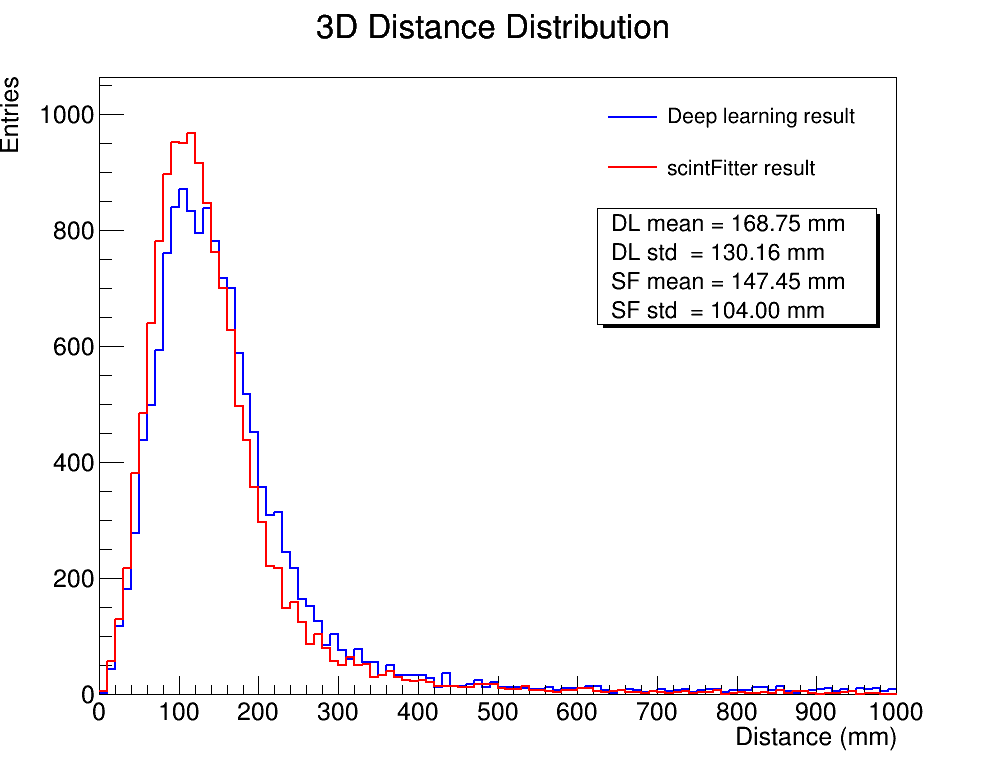
\includegraphics[width=0.8\textwidth]{figures/distance_distribution_comp.png}
    \caption{深度学习位置重建结果}
    \label{fig:position_reconstruction}
\end{figure}

从\ref{fig:position_reconstruction}中我们可以看到,
我们利用${}^{8}$B太阳中微子数据的验证集进行位置重建,
并选择了三维空间中预测的坐标与真实坐标之间的距离作为评价指标。
从图中我们可以看到,
深度学习模型的重建结果明显优于传统的重建方法,
同时在不同能量范围内,深度学习模型的重建结果也比较稳定。
而传统的重建方法在低能量范围内的重建结果较差,在能量较高时,重建结果较好。
这说明深度学习模型在不同能量范围内的重建结果都比较稳定。 
(如果最后训练出的结果满足,则使用这一表述,如不能则修改) 

\section{位置重建不确定性的量化}\label{sec:uncertainty}

上一节中我们介绍了SNO+探测器中位置重建的深度学习方法,
并给出了模型的架构和训练方法。在本节中,我们将之前提到的理论投入
实际应用,介绍如何具体量化这一深度学习位置重建模型的不确定性。

\subsection{粒子物理实验中不确定性的估计}

在正式开始量化深度学习模型的不确定性之前,我们首先要明确粒子物理实验领域和深度学习
领域UQ的类型以及两者的区别和联系。\cite{ParticleDataGroup:2024cfk}


在\ref{uncertainties}节中,我们了解到,深度学习领域中,
不确定性常被区分为偶然不确定性 (aleatoric uncertainty) 和
认知不确定性 (epistemic uncertainty) 。而它们与物理学中使用的概念
并非完全相同,存在视角上的差异。

首先,在数据收集与不确定性缩减方面,物理学通常关注在固定的实验设计下,
通过增加数据量来减少不确定性。在这种情况下,统计不确定性 (类似于偶然不确定性) 
会随着数据量的增加而减小,而系统不确定性 (类似于认知不确定性) 通常保持不变,
除非改进实验设计或进行更精确的校准。相比之下,深度学习领域更侧重于
通过收集不同类型的数据来改进模型本身,从而减少认知不确定性。他们所认为的“不可约减”
的偶然不确定性,是指在给定模型下的固有随机性。这种差异并非根本矛盾,
而是反映了不同领域关注点的侧重不同。

其次,“模型”的含义也有所不同。在物理学中,“模型”通常指代底层的物理过程或
通过模拟体现的探测器响应模型。系统不确定性或认知不确定性与对这些物理模型的
理解程度密切相关。而在机器学习领域,“模型”通常指训练得到的函数,
例如神经网络。认知不确定性常与训练后模型参数 $\theta$ 的不确定性相关联,
这种不确定性可以通过收集更多的训练数据来减少。这部分是因为机器学习任务
通常对数据生成过程 (如图像分类、自然语言处理) 的先验物理知识较少。

在与物理学 (特别是计算机模拟) 联系更紧密的 UQ 领域,
术语的划分更为细致,有助于减少歧义。UQ 领域通常区分以下几种不确定性
来源:
参数不确定性,例如模型中扰动参数 (nuisance parameters) 的不确定性;
结构不确定性,指模型本身与现实不符 (mismodelling) 导致的不确定性,例如在SNO+中
MC模拟与现实中探测器的实际情况的差异引起的不确定性;
算法不确定性,源于数值计算方法引入的误差,例如\ref{sec:classical_reconstruction}节中
提到的SNO+实际使用的Powell算法引入的不确定性;
实验不确定性,包括实验分辨率限制和统计涨落导致的不确定性;
以及插值不确定性,这是由于计算资源限制,在不同参数点之间进行插值而引入的不确定性。

\subsection{在深度学习中量化不确定性的方法}

深度学习中的不确定性分析方法在\ref{uncertainties}节中已经介绍过了,
我们这里使用的是MC Dropout方法和深度集成的方法来量化深度学习模型的不确定性。
量化的模型是在\ref{model_architecture}节中介绍的基于Transformer的模型。

对于MC Dropout方法,我们在训练时使用了Dropout层,
并在测试时使用了多次不同Dropout并进行前向传播来获得模型的预测分布。

对于深度集成方法,我们使用了多个模型,每个模型都使用了不同的随机种子进行训练,
然后将这些模型的预测结果进行平均,得到最终的预测分布。

\subsection{不确定性量化结果}

我们分别使用MC Dropout和深度集成方法对\ref{model_architecture}节中
描述的Transformer模型进行了不确定性量化。
对于MC Dropout,我们在训练期间使用的Dropout层在推理阶段保持启用状态。
通过对同一输入事件进行 $N$ 次前向传播 (每次使用不同的Dropout掩码) ,
我们得到了 $N$ 个不同的位置预测 
$\{\hat{\vec{x}}_1, \dots, \hat{\vec{x}}_N\}$。
最终的预测位置 $\hat{\vec{x}}$ 是这些预测的平均值,
而预测的不确定性则由这些预测的标准差或方差来估计。
这种方法估计的不确定性通常被认为是认知不确定性和偶然不确定性的混合。
对于深度集成方法,我们独立训练了 $M$ 个具有相同架构但使用不同随机
初始化种子和/或不同训练数据子集 (例如通过bootstrap) 的模型。
对于一个输入事件,每个模型 $m$ 产生一个预测 $\hat{\vec{x}}_m$。
最终的预测 $\hat{\vec{x}}$ 是 $M$ 个模型预测的平均值。
集成预测的方差 $\text{Var}(\{\hat{\vec{x}}_m\})$ 
主要量化了认知不确定性 (模型不确定性) 。
如果每个模型还被训练来预测其自身的不确定性
 (例如,预测位置分布的方差 $\sigma_m^2$) ,
则可以通过平均预测方差 $\frac{1}{M}\sum_m \sigma_m^2$ 来
估计偶然不确定性 (数据不确定性) 。

为了评估不确定性量化的质量,我们主要关注几个方面。
首先,一个好的不确定性估计应该与实际的预测误差相关,
即当模型预测的不确定性较高时,其预测误差也倾向于较大。
我们通过比较预测位置 $\hat{\vec{x}}$ 与真实位置 
$\vec{x}_{true}$ 的距离误差 $||\hat{\vec{x}} - \vec{x}_{true}||$ 
和模型预测的标准差 $\sigma_{pred}$ 来评估这一点。
其次,我们关注不确定性校准 (Calibration),
理想情况下,预测的不确定性应准确反映真实的误差水平,
例如,对于预测标准差为 $\sigma$ 的事件集合,
其预测位置的均方根误差 (RMSE) 应接近 $\sigma$。
我们通过绘制校准曲线 (比较不同预测不确定性分箱内的平均RMSE) 
来评估校准程度。此外,利用深度集成方法,我们可以尝试进行
不确定性分解,区分认知不确定性 
(来自模型本身,对应物理实验中的部分系统误差,
可通过更多数据或更好的模型减少) 和偶然不确定性 
(来自数据固有噪声,对应物理实验中的统计误差和部分系统误差,
通常难以减少) 。认知不确定性由集成成员预测之间的差异反映,
而偶然不确定性可由每个模型预测的平均方差反映 (如果模型输出方差) 。
最后,我们研究不确定性随物理量的变化,例如能量、
真实位置半径、PMT命中数等,这有助于理解模型在不同物理场景下的可靠性。

初步结果显示 (如图\ref{fig:uq_calibration}所示),
通过MC Dropout和深度集成方法得到的预测不确定性与实际的
预测误差表现出正相关性,表明模型在某种程度上能够识别其预测的置信度。
校准曲线显示,模型的不确定性估计在一定程度上是可靠的,
但可能存在过度自信或自信不足的区域,需要进一步的校准工作。

% \begin{figure}[htbp]
%     \centering
%     % Placeholder for actual figure file
%     \includegraphics[width=0.7\textwidth]{figures/uq_calibration_placeholder.png}
%     \caption{不确定性校准曲线示例:比较预测不确定性 (标准差) 与对应事件子集的实际均方根误差 (RMSE)。理想情况下,数据点应落在 $y=x$ 对角线上。}
%     \label{fig:uq_calibration}
% \end{figure}

如图\ref{fig:uq_vs_energy_radius}所示,
我们观察到预测的总不确定性通常在低能量和靠近探测器边缘的区域较高。
这符合预期,因为这些区域的可用信息较少或几何效应更复杂,
导致重建更具挑战性。深度集成方法的结果表明,
认知不确定性在训练数据覆盖不足或模型拟合能力有限的区域相对较高,
而偶然不确定性则更多地反映了光子统计和探测器响应的固有波动。

% \begin{figure}[htbp]
%     \centering
%     % Placeholder for actual figure file
%     \includegraphics[width=0.48\textwidth]{figures/uq_vs_energy_placeholder.png}
%     \includegraphics[width=0.48\textwidth]{figures/uq_vs_radius_placeholder.png}
%     \caption{预测不确定性随能量 (左) 和真实径向位置 (右) 的变化趋势示例。}
%     \label{fig:uq_vs_energy_radius}
% \end{figure}

这些量化的不确定性估计对于后续的物理分析至关重要。
例如,可以将事件按照其预测不确定性进行加权,
或者在进行信号和背景区分时,将具有高不确定性的事件排除或单独处理。
通过区分认知不确定性和偶然不确定性,我们可以更好地理解误差的来源:
高认知不确定性可能提示需要改进模型或收集更多样化的数据 
(对应减少模型相关的系统误差) ,而高偶然不确定性则反映了
实验本身的固有局限性 (对应统计误差和探测器相关的系统误差) 。
将这些基于深度学习的不确定性与传统方法 
(如MLE拟合中的参数误差) 进行比较,也是未来工作的一个重要方向。

